\documentclass[twocolumn]{article}
\usepackage[utf8]{inputenc}
\usepackage[spanish]{babel}
\usepackage{booktabs}
\usepackage{graphicx}
\usepackage{amsthm}
\usepackage[margin=1in]{geometry}
\usepackage{hyperref}
\usepackage[table]{xcolor}
\usepackage{bold-extra}

\theoremstyle{definition}
\newtheorem{indicador}{Indicador}
\newtheorem{recomendacion}{Recomendación}

\title{La base de datos \texttt{BDP-XFC} e indicadores para la profesionalización de ayudantes y profesores de asignatura de la Facultad de Ciencias de la UNAM}
\author{Leonardo Ignacio Martínez Sandoval\\Departamento de Matemáticas, Facultad de Ciencias, UNAM\\leomtz@ciencias.unam.mx}
\date{\today}
\begin{document}

\maketitle

\abstract{Los problemas de pago de ayudantes y profesores de asignatura de la UNAM han puesto en evidencia la existencia de diversos problemas administrativos. Debido a la pandemia causada por COVID-19, estos problemas llegaron a un punto intolerable. Esto generó un movimiento social para exigir soluciones.

Parte de las peticiones del movimiento contempla revisar aspectos de estabilidad laboral. Esto ha llevado a la generación de comisiones para estudiar el problema, y con ello a la necesidad de contar con datos para diagnosticarlo y proponer soluciones.

El sistema XFC de la Facultad de Ciencias de la UNAM almacena una gran cantidad de información relacionada con las labores de la dependencia. El acceso a esta base de datos es limitado debido a la naturaleza de la información contenida en él. Sin embargo, parte de la información es de interés general y es parcialmente pública a través de la página oficial de la Facultad de Ciencias. Pero no existe un mecanismo para acceder a ella fácilmente.

En este trabajo se documenta la creación de una base de datos de fácil acceso, \texttt{BDP-XFC}, a partir de la extracción de datos públicos de XFC. Se describe el mecanismo mediante el cual se extrajo la información. Además, se presenta un análisis de distintos indicadores útiles en el contexto de la profesionalización de ayudantes y profesores de asignatura.
}

\section{Contexto}

De manera histórica, los ayudantes y profesores de asignatura de la Facultad de Ciencias de la Universidad Nacional Autónoma de México han tenido inconvenientes en sus pagos \cite{appaa-problemas}. Estos van desde pagos que tardan meses en llegar, hasta prestaciones que no se pagan. Las causas dependen de muchos actores universitarios y es un problema complejo por resolver. En la Facultad de Ciencias de la UNAM, las autoridades han puesto en marcha distintos mecanismos para responder a la situación actual y prevenir que suceda nuevamente \cite{soluciones}.

La pandemia por COVID-19 intensificó el problema a un punto intolerable. La situación llevó fuertes cuestionamientos en torno a la figura de Profesor de Asignatura en la UNAM. Entre los aspectos discutidos, se encuentran aquellos de  profesionalización docente y estabilidad laboral.

Las relaciones entre la UNAM y su personal académico están regidas, entre otros documentos, por el Estatuto del Personal Académico (EPA) \cite{epa}. En él se establecen las figuras de Profesor de Tiempo Completo y Profesor de Asignatura. En un inicio, la figura de Profesor de Asignatura se pensó para profesionales que trabajaban fuera de una dependencia. Mediante contratos temporales, se incorporaban a la labor docente de las entidades para que la UNAM se enriqueciera de sus experiencias.

Sin embargo, en años recientes la figura de Profesor de Asignatura se ha reformulado en la práctica. Existe la percepción entre ciertos grupos de que gran parte de la carga docente recae en estas figuras. En parte, en este trabajo confirmamos cuantitativamente que este es el caso en la Facultad de Ciencias de la UNAM.

En términos de estabilidad laboral, el EPA contempla la figura de Profesor de Asignatura Definitivo. La definitividad es una cualidad que un profesor de asignatura puede obtener mediante un Concurso de Oposición Abierto para una o más materias. Los mecanismos para obtener estas definitividades, así como los derechos y obligaciones que se adquieren, se detallan en el EPA. Además, las definitividades otorgan derechos adicionales mediante el Contrato Colectivo del Trabajo (CCT) \cite{cct}. Si bien el EPA y el CCT son ambigüos en algunos aspectos, la Oficina de la Abogacía General de la UNAM ha establecido criterios de interpretación para varias de las dudas que surgen \cite{cri1,cri2}.

En el caso particular de la Facultad de Ciencias las definitividades son prácticamente inexistentes. Hoy en día no existen mecanismos bien definidos con respecto a ellas. No se cuenta con un procedimiento para determinar las necesidades de la dependencia en términos de profesores definitivos y tampoco se cuenta con procesos definidos para abrir y ejecutar concursos de oposición.

Este trabajo surge de la necesidad de contar con datos sólidos para que distintos miembros de la comunidad de la Facultad de Ciencias puedan estudiar el problema a detalle y proponer soluciones basadas en datos duros. En términos de acceso de la información, está respaldado por el punto XIX de las ``Obligaciones comunes a las Áreas Universitarias'' del Artículo 28 en las ``Normas en materia de transparencia y acceso a la información'' de la Universidad Nacional Autónoma de México \cite{transparencia}.


\section{El proyecto XFC y la base \texttt{BDP-XFC}}

La Facultad de Ciencias de la UNAM almacena información relacionada con sus labores a través del proyecto XFC. El acceso a la base de datos subyacente es limitado, pues contiene información personal y confidencial que se debe salvaguardar.

Sin embargo, dentro de esta base también hay mucha información relacionada con la labor docente de interés público para la comunidad. En particular, hay información acerca de las materias impartidas semestre tras semestre desde el año 2001. Esto incluye los grupos que se abrieron, los horarios, la cantidad de alumnos, los docentes que impartieron y con qué rol.

Esta información de interés para la comunidad se puede consultar mediante la página \url{http://fciencias.unam.mx}. Sin embargo, no es sencillo realizar consultas generales con este método.

Por esta razón, nuestro trabajo comienza con el diseño de una base de datos alternativa y de su llenado a partir de extracción de la información pública del sistema XFC. A esta base de datos le llamamos \texttt{BDP-XFC}, como acrónimo de ``base de datos pública tomada del proyecto XFC''.

En el Apéndice 1 definimos la estructura de \texttt{BDP-XFC}. Se explican las $6$ tablas que la conforman y sus relaciones. Además, para cada campo se explica de dónde se obtuvo la información. En la mayoría de los casos, esto se hizo mediante un script en Python que explorara repetidamente la página de la Facultad de Ciencias. Se tomó la precaución de no comprometer datos personales.

\section{Limitaciones}

La base de datos \texttt{BDP-XFC} tiene algunas limitaciones heredadas de XFC y algunas propias de nuestra forma de obtener la información.

Por un lado, estamos limitados hacia atrás en el tiempo. La base XFC tiene información de la docencia de la Facultad de Ciencias únicamente a partir del semestre 2001-1.

Por otro lado, cierta información de la base XFC depende de la actualización de datos personales, que no necesariamente está al día. Esto afecta la veracidad de registros individuales. Sin embargo, para la mayoría de análisis que presentamos este es un problema menor.

En términos de las limitaciones de nuestro método, la página de la Facultad de Ciencias no muestra el histórico de nombramientos de cada académico, sino únicamente el último que obtuvo. Es posible que la base XFC sí un histórico que haga el análisis más informativo, pero que no esté abierto al público todavía.

Aunado a eso, la página no muestra de manera pública las solicitudes de impartir cursos, aunque estas sí estén disponibles en XFC. Una versión anonimizada de esta información podría generar conclusiones interesantes sobre las necesidades docentes de la Facultad de Ciencias y a la vez proteger la identidad de los solicitantes.

\section{Construcción de indicadores}

Si bien el problema actual concierne a profesores de asignatura y ayudantes, en este primer trabajo nos enfocamos en la figura de Profesores de Asignatura, es decir, sólo usaremos las entidades de la tabla \texttt{teaching} en donde el campo \texttt{ProfType} sea Profesor.

También, simplificaremos todavía más el campo \texttt{SimpAppointment} de la tabla \texttt{profs}. Sólo haremos distinción entre si el profesor es de asignatura, es decir si el valor es \texttt{PA}, o si no. Dentro de la Facultad de Ciencias esto es prácticamente equivalente a separar a los docentes entre Profesores de Asignatura sin definitividad, y personal académico de carrera.

En todo el análisis es importante tener en cuenta que la labor docente de la Facultad de Ciencias se realiza en periodos semestrales, mientras que el ingreso a las licenciaturas es anual. Esto hace que los semestres pares tengan un comportamiento distinto al de los semestres impares. Además, en nuestro análisis descartaremos los periodos intersemestrales en los que se ofrecen clase pues usualmente se abren muy pocos grupos en estos periodos.

\subsection{Indicadores históricos}

Comenzamos estudiando algunas tendencias históricas de la información.

\begin{figure}
    \centering
    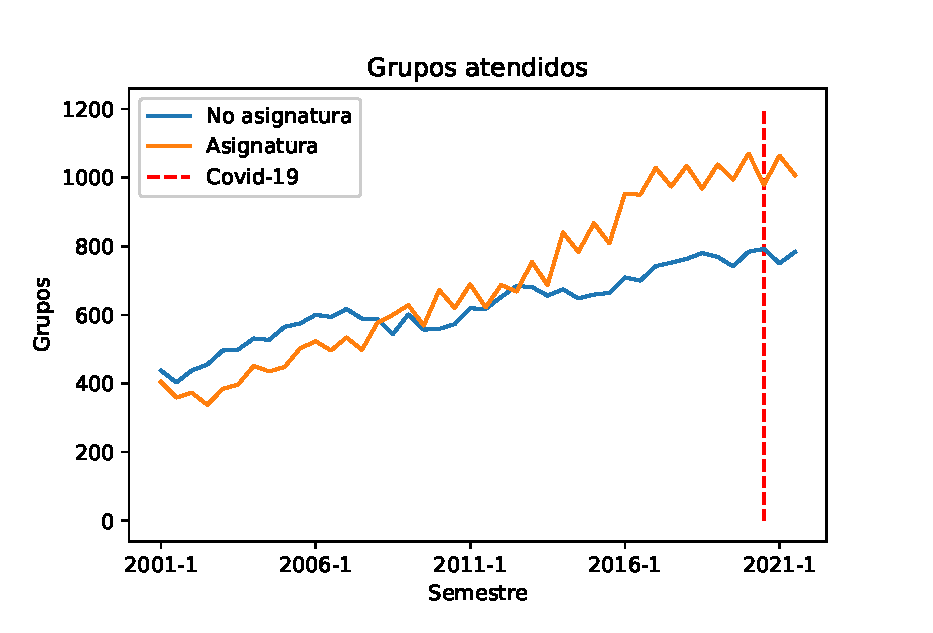
\includegraphics[width=0.5\textwidth]{fig/grupos.eps}
    \caption{Grupos atendidos}
    \label{fig:groups}
\end{figure}


\begin{figure}
    \centering
    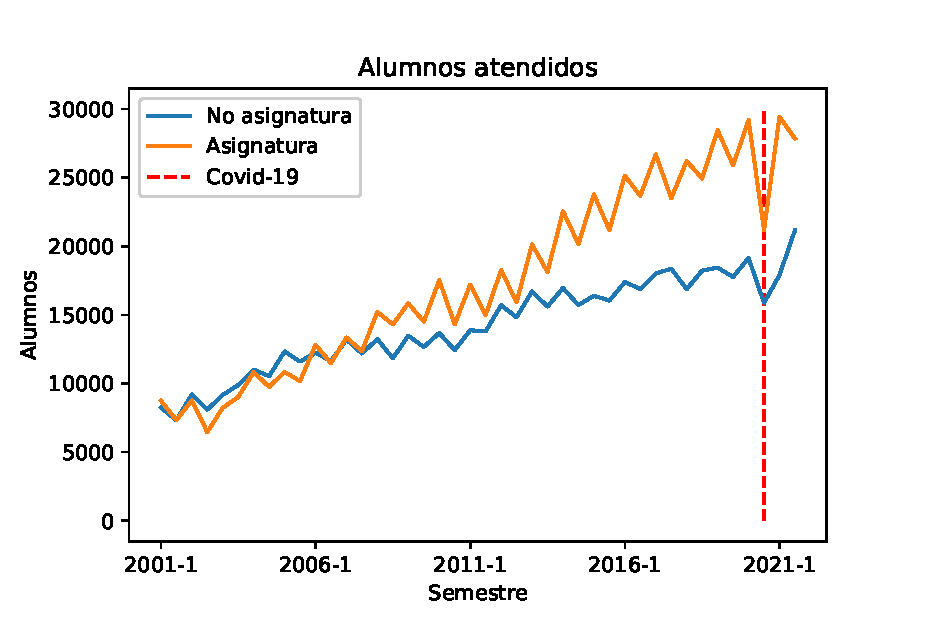
\includegraphics[width=0.5\textwidth]{fig/alumnos.eps}
    \caption{Alumnos atendidos}
    \label{fig:students}
\end{figure}


La gráfica en la Figura \ref{fig:groups} muestra la cantidad de grupos atendidos por ambas clases de personal académico desde el semestre 2001-1. La gráfica en la Figura \ref{fig:students} muestra la cantidad de alumnos (con repetición) atendidos por ambas clases de personal académico desde el semestre 2001-1.

En ambos casos, notamos que la labor de los Profesores de Asignatura ha aumentado considerablemente. Esto confirma a partir de los datos que, en efecto, se hace uso de la figura de Profesor de Asignatura mucho más que anteriormente.

En la figura correspondiente a grupos, llaman en particular la atención los semestres 2014-1, 2016-1 y 2017-1. En ellos se observa que el aumento de grupos impartidos por profesores de asignatura tuvo un aumento local mayor al de otros semestres.

Otra información de esta figura es que la asignación de grupos para personal de carrera es estable con respecto a la paridad del semestre. Por otro lado, la asignación de grupos para profesores de asignatura tiene oscilaciones de acuerdo a si el semestre es par o impar, siendo menor en el segundo de los casos.

En el caso del semestre 2020-2 observamos una fuerte deserción de alumnos, atribuible a la pandemia por COVID-19 y al periodo de bajas adicional que se abrió. Este fenómeno no se detecta en los datos por grupos. Una posible explicación es que no hubo un mecanismo formal para que un profesor dejara de impartir clases.

\subsection{Menor cantidad de grupos de asignatura por materia}

El EPA establece que las definitividades de Profesores de Asignatura se establecen por materia. Además, indica que los concursos de oposición abiertos para obtener esta cualidad se deben abrir de acuerdo a las necesidades de cada dependencia.

Con esto en mente, esta sección propone algunos indicadores que pueden ayudar a entender la necesidad de abrir concursos de oposición en ciertas materias. Dejaremos el punto de vista histórico y nos enfocaremos únicamente a la información correspondiente a los últimos 5 años (10 semestres), esto es, de 2017-1 a 2021-2.

De esta manera, realizamos un análisis similar al de la sección anterior, pero filtrando por materia y periodo de tiempo. Como ejemplo de esto, tomamos el curso Cálculo Diferencial e Integral I y generamos la Figura \ref{fig:calcgroups} y la Figura \ref{fig:calcstudents}.

\begin{figure}
    \centering
    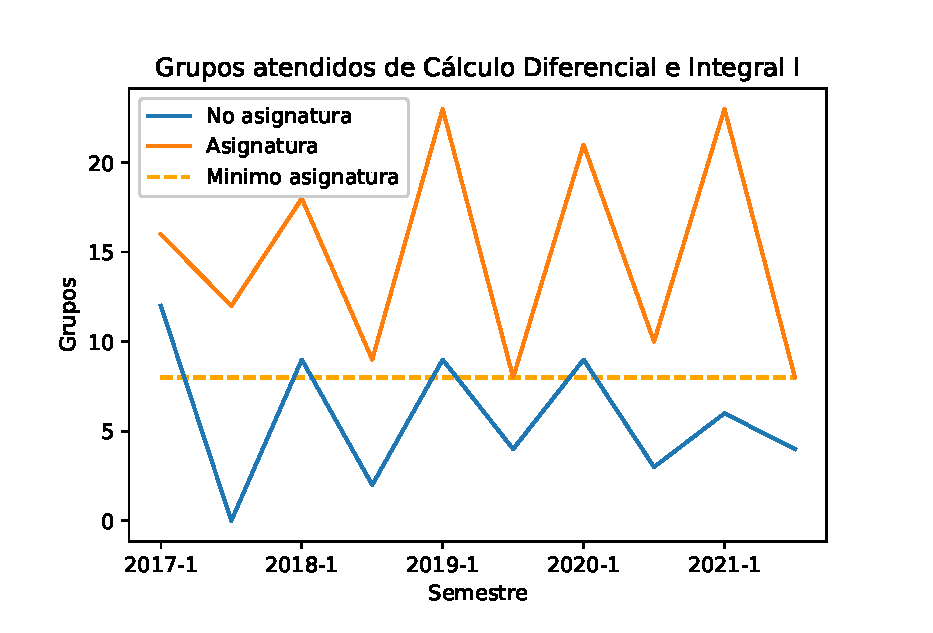
\includegraphics[width=0.5\textwidth]{fig/calculo_grupos.eps}
    \caption{Grupos de CDI I atendidos}
    \label{fig:calcgroups}
\end{figure}


\begin{figure}
    \centering
    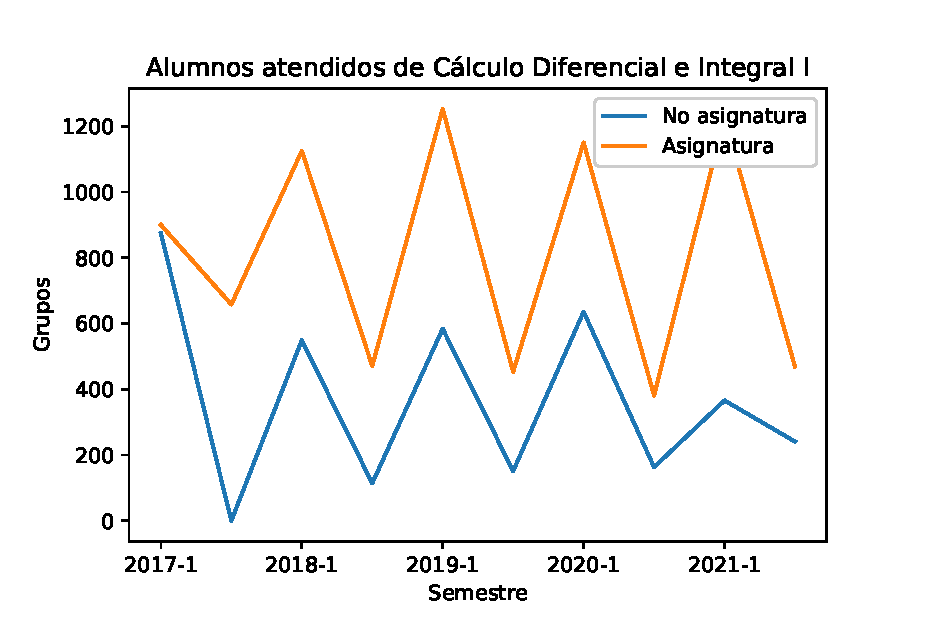
\includegraphics[width=0.5\textwidth]{fig/calculo_alumnos.eps}
    \caption{Alumnos de CDI I atendidos}
    \label{fig:calcstudents}
\end{figure}

Las figuras presentan una oscilación de acuerdo al semestre. Es normal que tengamos picos hacia arriba en semestres impares, pues la materia corresponde al primer semestre de varias licenciaturas de la Facultad de Ciencias.

Otra observación es que en todos los semestres, sin importar su paridad, la materia se encuentra atendida principalmente por profesores de asignatura, tanto en número de grupos, como de alumnos. En el semestre 2017-2 la materia no fue impartida por ningún docente de carrera.

La línea punteada horizontal muestra nuestro primer indicador. 

\begin{indicador} Para una materia dada, definimos $\alpha$ como el mínimo número de grupos dirigidos por profesores de asignatura en los últimos 10 semestres.
\end{indicador}

 El valor $\alpha$ es importante pues habla de que en cada uno de los semestres de este periodo se han necesitado al menos $\alpha$ profesores de asignatura para impartir la materia. En Cálculo Diferencial e Integral I este valor es $8$.
 
 \subsection{Profesores de asignatura que imparten una misma materia repetidamente}

La figura de la sección anterior no garantiza que los profesores de asignatura que imparten Cálculo Diferencial e Integral I siempre sean los mismos. Es importante medir esto pues las personas que ocupan puestos de Profesor de Asignatura no necesariamente quieren continuar en él de manera indefinida. En ocasiones sólo imparten una materia durante algunos años con el fin de continuar su preparación académica y posteriormente se integran a otra rama del campo laboral.

Esto nos lleva a la siguiente pregunta. Para una materia dada, de los profesores de asignatura que la impartieron, ¿cuántas veces la impartieron? Como respuesta a esto, veamos la distribución de dichos valores. Tomemos de nuevo Cálculo Diferencial e Integral I como ejemplo. La Figura \ref{fig:calchist} muestra dicha distribución.

\begin{figure}
    \centering
    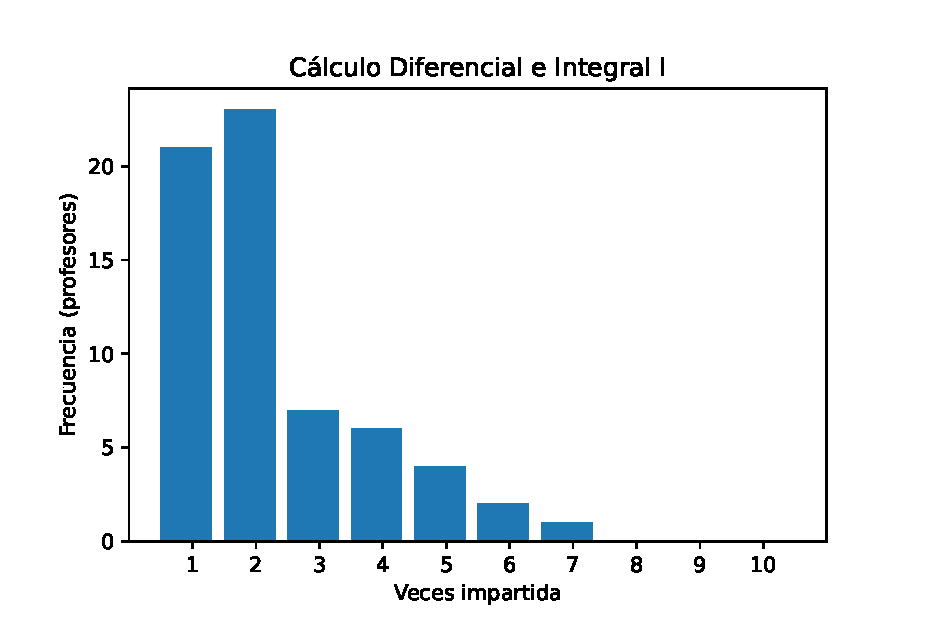
\includegraphics[width=0.5\textwidth]{fig/dist_calculo.eps}
    \caption{Distribución de veces que se imparte una materia}
    \label{fig:calchist}
\end{figure}

La última barra indica que hay un profesor de asignatura que impartió la materia en 7 de los 10 semestres analizados. La penúltima muestra que hay dos que la impartieron 6 veces. Así mismo, hay cuatro que la impartieron 5 veces. Es posible que estos siete profesores estén interesados en obtener una definitividad en la materia.

En el caso de los profesores que impartieron la materia 4 veces o menos, no es totalmente claro que les interese obtener una definitividad. Sin embargo, dentro de los que sí, es más posible que estén siguiendo una estrategia de impartir alternadamente Cálculo Diferencial e Integral I y luego Cálculo Diferencial e Integral II (y sus continuaciones). Es posible que estos profesores estén interesados en obtener definitividad en ambas materias (o más) para poder impartirlas alternadamente. Entender este fenómeno requiere de un análisis más profundo, que no hacemos aquí, pero que también puede obtenerse a partir de la información en \texttt{BDP-XFC}.

La discusión en los dos párrafos anteriores nos lleva a nuestro segundo indicador.

\begin{indicador}
    Para una materia, llamamos $\beta$ a la cantidad de profesores de asignatura que han impartido esa materia $5$ o más veces en los últimos $10$ semestres.
\end{indicador}
 
\section{Uso de indicadores}

Regresemos a la pregunta: para una materia dada ¿cuántas definitividades es conveniente abrir? Hay varios factores que se deben tomar en cuenta. Sin embargo, los indicadores $\alpha$ y $\beta$ ayudan a responder esto de dos maneras distintas.

Por un lado, el valor de $\alpha$ está relacionado con las necesidades en términos de la Facultad de Ciencias: nos dice que para una materia dada, esa cantidad de grupos de profesores de asignatura siempre se han abierto en los últimos 10 semestres. Su valor no depende de la paridad del semestre.

Por otro lado, el valor de $\beta$ está relacionado con las necesidades en términos de los docentes: nos habla de cuántos docentes han dado la materia tantas veces que podría interesarles obtener una definitividad.

Nuestro último paso es construir una tabla que resuma estos indicadores. Con el fin de tener un análisis más puntual, nos enfocaremos únicamente en las materias obligatorias de cada una de las licenciaturas que imparte la Facultad de Ciencias en Ciudad Universitaria. Tomaremos únicamente los planes de estudio más recientes de cada una de ellas.

Para cada una de estas materias, tomaremos únicamente aquellas en las que $\alpha\geq 3$. Esta condición está pensada en dar un margen para la apertura de definitividades y que además haya la garantía de tener por lo menos dos espacios para la rotación de personal académico. Una última decisión que tomamos fue la de eliminar de la tabla las materias Taller Nivel 1, 2, 3, 4 correspondientes a la licenciatura en biología, pues la forma en que se imparten y se registran sus profesores es muy particular.

En el Cuadro \ref{tab:obli} (al final del documento), se puede ver el valor de $\alpha$, el de $\beta$ y en qué licenciaturas la materia es obligatoria. Los valores están ordenados de manera descendiente por la columna $\alpha$. Este es un muy buen punto de partida para decidir cuántos concursos de definitividad abrir para cada una de estas materias.

\section{Conclusiones y recomendaciones}

En el trabajo construimos una versión pequeña de la base que subyace al proyecto XFC conformada únicamente de información pública y de interés general. Le llamamos \texttt{BDP-XFC}. Vimos que dicha base de datos nos puede dar información valiosa acerca de la vida académica de la Facultad de Ciencias de la UNAM.

En particular, a partir de ella construimos indicadores para analizar la pertinencia de abrir Concursos de Oposición Abiertos para definitividades de profesores de asignatura. Cada una de las materias en el Cuadro \ref{tab:obli} requiere de varios profesores de asignatura para ser impartida cada semestre, lo cual es un punto inicial para considerar la apertura de definitividades. Además, la tabla cuenta con la cantidad de profesores a quienes les podría interesar solicitar la apertura de dichos concursos.

\begin{recomendacion}

Generar discusiones colegiadas acerca de las materias en el Cuadro \ref{tab:obli} que consideren el valor de $\beta$ y otros criterios académicos como: perfil del docente que imparte la materia, particularidades de la materia, beneficio de renovación docente en la materia, etc.

\end{recomendacion}

La paridad del semestre es fundamental en la vida académica de la Facultad. Sería importante entender aquellos aspectos de esta oscilación que estén relacionados con la problemática de los profesores de asignatura y ayudantes. Este estudio también dará luz hacia la pertinencia de otorgar definitividades a una misma persona en más de una materia.

\begin{recomendacion}

Proponer y usar indicadores sensibles a la paridad de los semestres.

\end{recomendacion}

La base \texttt{BDP-XFC} resultó útil. Sin embargo, también notamos que cuenta con limitaciones debido a que fue obtenida mediante la extracción de información pública, y no de consultas directas a XFC.

\begin{recomendacion}
Comenzar dentro de la Facultad de Ciencias un esfuerzo institucional para poner a disposición de la comunidad toda la información pública de la vida académica de la Facultad. Este esfuerzo debe incluir mecanismos de fácil acceso a información agregada y consideraciones de privacidad de los individuos. 
\end{recomendacion}

Este acercamiento de uso de la información es un primer paso hacia la toma de decisiones más informadas, transparentes y abiertas.

\begin{recomendacion}

Extender fuertemente el uso de datos en la toma de decisiones de la Facultad de Ciencias. Incluir a toda la comunidad en propuestas del uso de \texttt{BDP-XFC} para la toma de decisiones.

\end{recomendacion}

\bibliographystyle{plain}
\bibliography{refs}

\section*{Apéndice: Definición de la base \texttt{BDP-XFC}}

La base de datos \texttt{BDP-XFC} está conformada por seis tablas y cinco relaciones entre campos. En la Figura \ref{fig:estructura} se muestra un diagrama de la estructura. En las subsecciones siguientes se detallan las tablas, los campos y las relaciones.

\begin{figure}
    \centering
    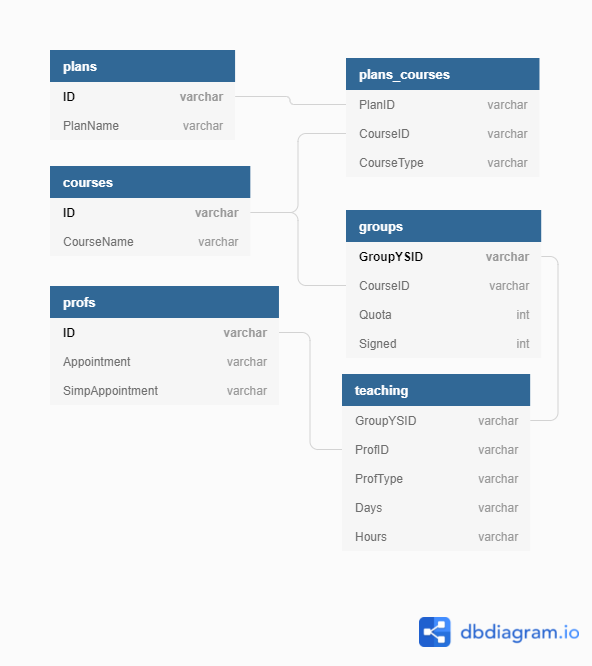
\includegraphics[width=0.5\textwidth]{fig/DB-relations.png}
    \caption{Estructura de la base de datos \texttt{BDP-XFC}.}
    \label{fig:estructura}
\end{figure}

\subsection{\texttt{plans}} 

Las instancias corresponden a los planes más actuales de la licenciatura de la Facultad de Ciencias. Sus campos son:

\begin{itemize}
    \item \texttt{\textbf{ID}} - Es la clave de la licenciatura correspondiente de acuerdo al sistema XFC.
    \item \texttt{PlanName} - Es el nombre de la licenciatura correspondiente de acuerdo al sistema XFC.
\end{itemize}

\subsection{\texttt{courses}} 

Las instancias corresponden a materias de la Facultad de Ciencias. Sus campos son:

\begin{itemize}
    \item \texttt{\textbf{ID}} - Es la clave de materia de acuerdo al sistema XFC.
    \item \texttt{CourseName} - Es el nombre de la materia de acuerdo al sistema XFC.
\end{itemize}

\subsection{\texttt{groups}}

Las instancias corresponden a los grupos para todas las materias que ha habido desde 2001-1. Sus campos son:

\begin{itemize}
    \item \texttt{\textbf{GroupYSID}} - Es un número de identificación único que contiene la materia del grupo, la clave del grupo, el año y semestre en que se impartió.
    \item \texttt{Quota} - Es el cupo de grupo de acuerdo al sistema XFC.
    \item \texttt{Signed} - Es la cantidad de alumnos inscritos de acuerdo al sistema XFC.
\end{itemize}

\subsection{\texttt{profs}}

Las instancias corresponden a los académicos que han impartido alguna clase desde el semestre 2001-1. Se tomaron precauciones para anonimizar esta tabla y dejar fuera datos sensibles. Sus campos son:

\begin{itemize}
    \item \texttt{\textbf{ID}} - Es el número de identificación en el directorio de personal de XFC.
    \item \texttt{Appointment} - Es el nombramiento que tiene el profesor al día de la extracción de la información de XFC.
    \item \texttt{SimpAppointment} - Es una versión simplificada del campo anterior, con menos categorías. Sus posibles valores son:
    \begin{itemize}
        \item Ayud - Ayudante
        \item Inv - Investigador
        \item PA - Profesor de asignatura
        \item PTC - Profesor de tiempo completo
        \item PMT - Profesor de medio tiempo
        \item Tec - Técnico académico
        \item ND - Información no disponible
    \end{itemize}
\end{itemize}

\subsection{\texttt{teaching}}

Las instancias son relaciones de qué académico impartió qué cursos, así como otros datos de utilidad. Sus campos son:

\begin{itemize}
    \item \texttt{ProfID} - El número de identificación del académico.
    \item \texttt{GroupYSID} - El número de identificación del grupo.
    \item \texttt{ProfType} - El rol que tuvo el académico en el grupo. Puede ser:
    \begin{itemize}
        \item Ayud. Lab.
        \item Ayudante
        \item Calificador
        \item Discusión
        \item Laboratorio
        \item Profesor
    \end{itemize}
    \item \texttt{Days} - Días en los que el profesor imparte en el grupo.
    \item \texttt{Hours} - Horas en las que el profesor imparte en el grupo.
\end{itemize}

\subsection{\texttt{plans\_courses}}
Las instancias son las relaciones entre planes de estudio y materias. Sus campos son:

\begin{itemize}
    \item \texttt{CourseID} - El número de identificación de la materia.
    \item \texttt{PlanID} - El número de identificación del curso.
    \item \texttt{CourseType} - Si la materia es optativa u obligatoria.
\end{itemize}

\subsection{Relaciones}

Los campos de las tablas comparten las siguientes relaciones:

\begin{itemize}
    \item El campo \texttt{ID} de \texttt{plans} tiene una relación uno a muchos con el campo \texttt{PlanID} de \texttt{plans\_courses}.
    
    \item El campo \texttt{ID} de \texttt{courses} tiene una relación uno a muchos con el campo \texttt{CourseID} de \texttt{plans\_courses}.
    
    \item El campo \texttt{GroupYSID} de \texttt{courses} tiene una relación uno a muchos con el campo \texttt{GroupYSID} de \texttt{teaching}.
    
    \item El campo \texttt{ID} de \texttt{profs} tiene una relación uno a muchos con el campo \texttt{ProfID} de \texttt{teaching}.
    
    \item El campo \texttt{ID} de \texttt{courses} tiene una relación uno a muchos con el campo \texttt{CourseID} de \texttt{groups}.
    
\end{itemize}

\onecolumn

\onecolumn
\begin{table}[h!]
\centering
\begin{tabular}{l|ll|llllllll}
\textbf{Materia}             & $\alpha$ & $\beta$             & \textbf{A}        & \textbf{CC}        & \textbf{F}        & \textbf{M}        & \textbf{CT}        & \textbf{FB}        & \textbf{MA}        & \textbf{B}        \\\hline
Biología de Animales II      & 17       & 9                   &                     &                     &                     &                     &                     &                     &                     & \cellcolor{blue!25} \\
Biotecnología I              & 17       & 7                   &                     &                     &                     &                     &                     &                     &                     & \cellcolor{blue!25} \\
Ciencias de la Tierra        & 15       & 8                   &                     &                     &                     &                     &                     &                     &                     & \cellcolor{blue!25} \\
Evolución I                  & 14       & 9                   &                     &                     &                     &                     &                     &                     &                     & \cellcolor{blue!25} \\
Biogeografía I               & 13       & 5                   &                     &                     &                     &                     &                     &                     &                     & \cellcolor{blue!25} \\
Bioestadística               & 12       & 10                  &                     &                     &                     &                     &                     &                     &                     & \cellcolor{blue!25} \\
Biología de Animales III     & 12       & 8                   &                     &                     &                     &                     &                     &                     &                     & \cellcolor{blue!25} \\
BMC II                       & 12       & 7                   &                     &                     &                     &                     &                     &                     &                     & \cellcolor{blue!25} \\
Genética I                   & 12       & 8                   &                     &                     &                     &                     &                     &                     &                     & \cellcolor{blue!25} \\
Biología de Plantas I        & 11       & 6                   &                     &                     &                     &                     &                     &                     &                     & \cellcolor{blue!25} \\
Ecología I                   & 11       & 6                   &                     &                     &                     &                     &                     &                     &                     & \cellcolor{blue!25} \\
Biología de Hongos           & 10       & 8                   &                     &                     &                     &                     &                     &                     &                     & \cellcolor{blue!25} \\
Paleobiología                & 10       & 5                   &                     &                     &                     &                     &                     &                     &                     & \cellcolor{blue!25} \\
Química Orgánica             & 10       & 5                   &                     &                     &                     &                     &                     &                     &                     & \cellcolor{blue!25} \\
Biología de Plantas II       & 9        & 8                   &                     &                     &                     &                     &                     &                     &                     & \cellcolor{blue!25} \\
BMC I                        & 9        & 10                  &                     &                     &                     &                     &                     &                     &                     & \cellcolor{blue!25} \\
Biología de Animales I       & 8        & 6                   &                     &                     &                     &                     &                     &                     &                     & \cellcolor{blue!25} \\
BMC III                      & 8        & 4                   &                     &                     &                     &                     &                     &                     &                     & \cellcolor{blue!25} \\
CDI I                        & 8        & 7                   & \cellcolor{blue!25} &                     & \cellcolor{blue!25} & \cellcolor{blue!25} &                     &                     & \cellcolor{blue!25} &                     \\
Geometría Analítica I        & 8        & 5                   & \cellcolor{blue!25} &                     & \cellcolor{blue!25} & \cellcolor{blue!25} &                     &                     & \cellcolor{blue!25} &                     \\
Recursos Naturales           & 8        & 0                   &                     &                     &                     &                     &                     &                     &                     & \cellcolor{blue!25} \\
Álgebra Lineal I             & 7        & 3                   & \cellcolor{blue!25} & \cellcolor{blue!25} & \cellcolor{blue!25} & \cellcolor{blue!25} &                     &                     & \cellcolor{blue!25} &                     \\
Álgebra Superior II          & 7        & 0                   & \cellcolor{blue!25} & \cellcolor{blue!25} &                     & \cellcolor{blue!25} &                     &                     & \cellcolor{blue!25} &                     \\
CDI II                       & 7        & 2                   & \cellcolor{blue!25} &                     & \cellcolor{blue!25} & \cellcolor{blue!25} &                     &                     & \cellcolor{blue!25} &                     \\
CDI III                      & 7        & 0                   & \cellcolor{blue!25} &                     & \cellcolor{blue!25} & \cellcolor{blue!25} &                     &                     & \cellcolor{blue!25} &                     \\
Ecuaciones Diferenciales I   & 7        & 5                   & \cellcolor{blue!25} &                     & \cellcolor{blue!25} & \cellcolor{blue!25} &                     &                     & \cellcolor{blue!25} &                     \\
CDI IV                       & 6        & 2                   & \cellcolor{blue!25} &                     & \cellcolor{blue!25} & \cellcolor{blue!25} &                     &                     & \cellcolor{blue!25} &                     \\
Álgebra Superior I           & 5        & 2                   & \cellcolor{blue!25} & \cellcolor{blue!25} &                     & \cellcolor{blue!25} &                     &                     & \cellcolor{blue!25} &                     \\
Biología de Procariontes     & 5        & 10                  &                     &                     &                     &                     &                     &                     &                     & \cellcolor{blue!25} \\
Geometría Analítica II       & 5        & 2                   & \cellcolor{blue!25} &                     & \cellcolor{blue!25} & \cellcolor{blue!25} &                     &                     & \cellcolor{blue!25} &                     \\
Pensiones Privadas           & 5        & 5                   & \cellcolor{blue!25} &                     &                     &                     &                     &                     &                     &                     \\
Química                      & 5        & 9                   &                     &                     &                     &                     &                     &                     &                     & \cellcolor{blue!25} \\
Sistemática I                & 5        & 6                   &                     &                     &                     &                     &                     &                     &                     & \cellcolor{blue!25} \\
Economía                     & 4        & 7                   & \cellcolor{blue!25} &                     &                     &                     &                     &                     &                     &                     \\
Análisis Matemático I        & 3        & 0                   & \cellcolor{blue!25} &                     &                     & \cellcolor{blue!25} &                     &                     & \cellcolor{blue!25} &                     \\
Demografía                   & 3        & 5                   & \cellcolor{blue!25} &                     &                     &                     &                     &                     &                     &                     \\
Fenómenos Colectivos         & 3        & 2                   &                     &                     & \cellcolor{blue!25} &                     & \cellcolor{blue!25} & \cellcolor{blue!25} &                     &                     \\
Investigación de Operaciones & 3        & 7                   & \cellcolor{blue!25} &                     &                     &                     &                     &                     & \cellcolor{blue!25} &                     \\
MASP II                      & 3        & 3                   & \cellcolor{blue!25} &                     &                     &                     &                     &                     &                     &                     \\
Matemáticas Financieras      & 3        & 3                   & \cellcolor{blue!25} &                     &                     &                     &                     &                     &                     &                     \\
Probabilidad I               & 3        & 5                   & \cellcolor{blue!25} & \cellcolor{blue!25} &                     &                     &                     &                     & \cellcolor{blue!25} &                     \\
Probabilidad II              & 3        & 1 & \cellcolor{blue!25} &                     &                     &                     &                     &                     & \cellcolor{blue!25} &                     \\
Procesos Estocásticos I      & 3        & 1 & \cellcolor{blue!25} &                     &                     &                     &                     &                     & \cellcolor{blue!25} &                    
\end{tabular}
\caption{Tabla de valores de $\alpha$ y $\beta$}
\label{tab:obli}
\end{table}
\twocolumn


\end{document}